\chapter{Consensus Algorithms Exercise 1}
\assignment{
  \textbf{Exercise 1} \\
  Let the graphs $G_1$, $G_2$, and $G_3$ be given as shown in Figure \ref{fig:consensus1}.
  \begin{enumerate}
  \item Derive the graphs $G_1 = (V_1, E_1)$, $G_2 = (V_2, E_2)$, and $G_3 = (V_3, E_3)$.
  \item Derive the Laplacian matrices of the graphs.
  \item Let $G_1$, $G_2$, and $G_3$ be the topology of a network of agents with integrator dynamics and consensus
    protocol
    \begin{equation}
      u_i = \sum_{j\in N_i} \left( x_j - x_i \right)
      \label{eq:coneqdyn1}
    \end{equation}
    Will the agents reach consensus, and if so, what type of consensus
    (consensus/average-consensus/min-consensus/max-consensus)?
  \end{enumerate}
  
  \begin{figure}[H]
    \centering
    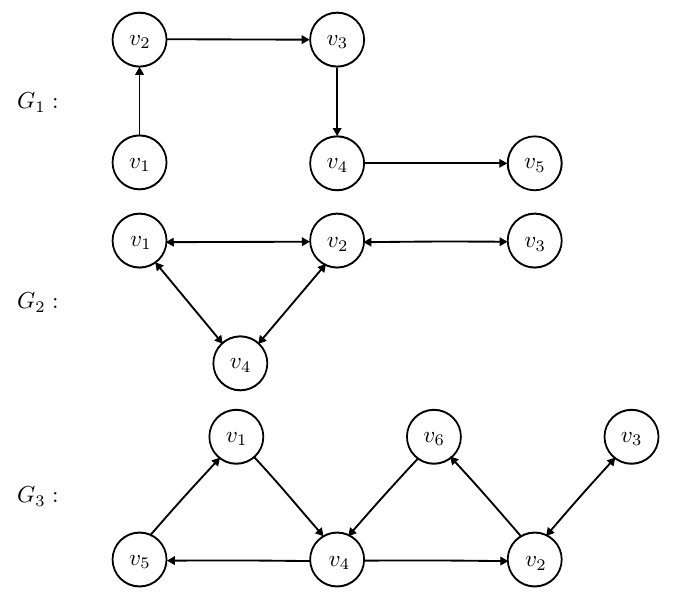
\includegraphics[width=0.8\textwidth]{consensus_fig1.png}
    \caption{Illustration of a dynamic graph.}
    \label{fig:consensus1}
  \end{figure}
}

\assignment{
  \textbf{Exercise 2} \\
  Consider the two graphs $G_1 = (V_1, E_1)$ and $G_2 = (V_2, E_2)$, where \\
  $V_1 = \left\{v_1, v_2, v_3, v_4\right\},\, V_2 = \left\{v_1, v_2, v_3 , v_4 , v_5, v_6 \right\},$ \\
  $E_1 = \left\{e_{12}, e_{21} , e_{23}, e_{32}, e_{24}, e_{42}, e_{34}, e_{43}, e_{14}, e_{41} \right\},$ \\
  $E_2 = \left\{e_{12} , e_{23} , e_{31}, e_{14} , e_{41} , e_{43}, e_{36} , e_{65} , e_{54} \right\}.$ \\
  \begin{enumerate}
  \item Derive the convergence rate of the disagreement of the two dynamic networks with topology G1 and G2 and agents
    governed by integrator dynamics consensus protocol in equation \eqref{eq:coneqdyn1}.
  \item Simulate the dynamic networks and compare the simulated results with the convergence bound.
  \end{enumerate}
}

\assignment{
  \textbf{Exercise 3} \\
  The graph $G = (V, E)$ with vertices $V = \{v_1, v_2, v_3, v_4 , v_5 \}$ and edges $E = \{e_{12} , e_{23}, e_{34} ,
  e_{45} \}$ reaches consensus with consensus protocol \eqref{eq:coneqdyn1}. Modify the consensus algorithm such that the network
  converges to
  \begin{equation}
    \begin{bmatrix}
      x_1 - x_2 \\
      x_2 - x_3 \\
      x_3 - x_4 \\
      x_4 - x_5
    \end{bmatrix}
    =
    \begin{bmatrix}
      1 \\
      3 \\
      9 \\
      2
    \end{bmatrix}
  \end{equation}
}

\assignment{
  \textbf{Exercise 4} \\
 Add a virtual agent to the dynamic network in Figure \ref{fig:consensus2} such that the state of every agent follows
 the constant reference of the virtual agent.
 \begin{figure}[H]
   \centering
   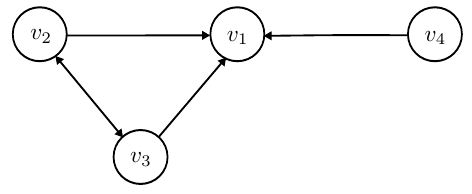
\includegraphics[width=0.5\textwidth]{consensus_fig2.png}
   \caption{Illustration of a dynamic graph}
   \label{fig:consensus2}
 \end{figure}

}
